\documentclass[11pt]{article}
\usepackage{amsmath}
\usepackage{amssymb}
\usepackage{wasysym}

\usepackage[dvipsnames]{xcolor}
\usepackage[colorlinks=true, urlcolor=NavyBlue]{hyperref}
\usepackage{url}
\usepackage{graphicx}
\usepackage{inconsolata}
\title{Homework 0}
\author{Your name here}
\date{\today{}}

\begin{document}
\maketitle

\section{Exercise 1}

Given $f(x) = x^n$, what is $\frac{df}{dx}$?

\subsection*{Solution}

\begin{align}
    \frac{df}{dx} = nx^{n-1}
\end{align}

\section{Exercise 2}

% Add an image of the Mona Lisa here.

\subsection*{Solution}

%\begin{figure}
    %\centering
    %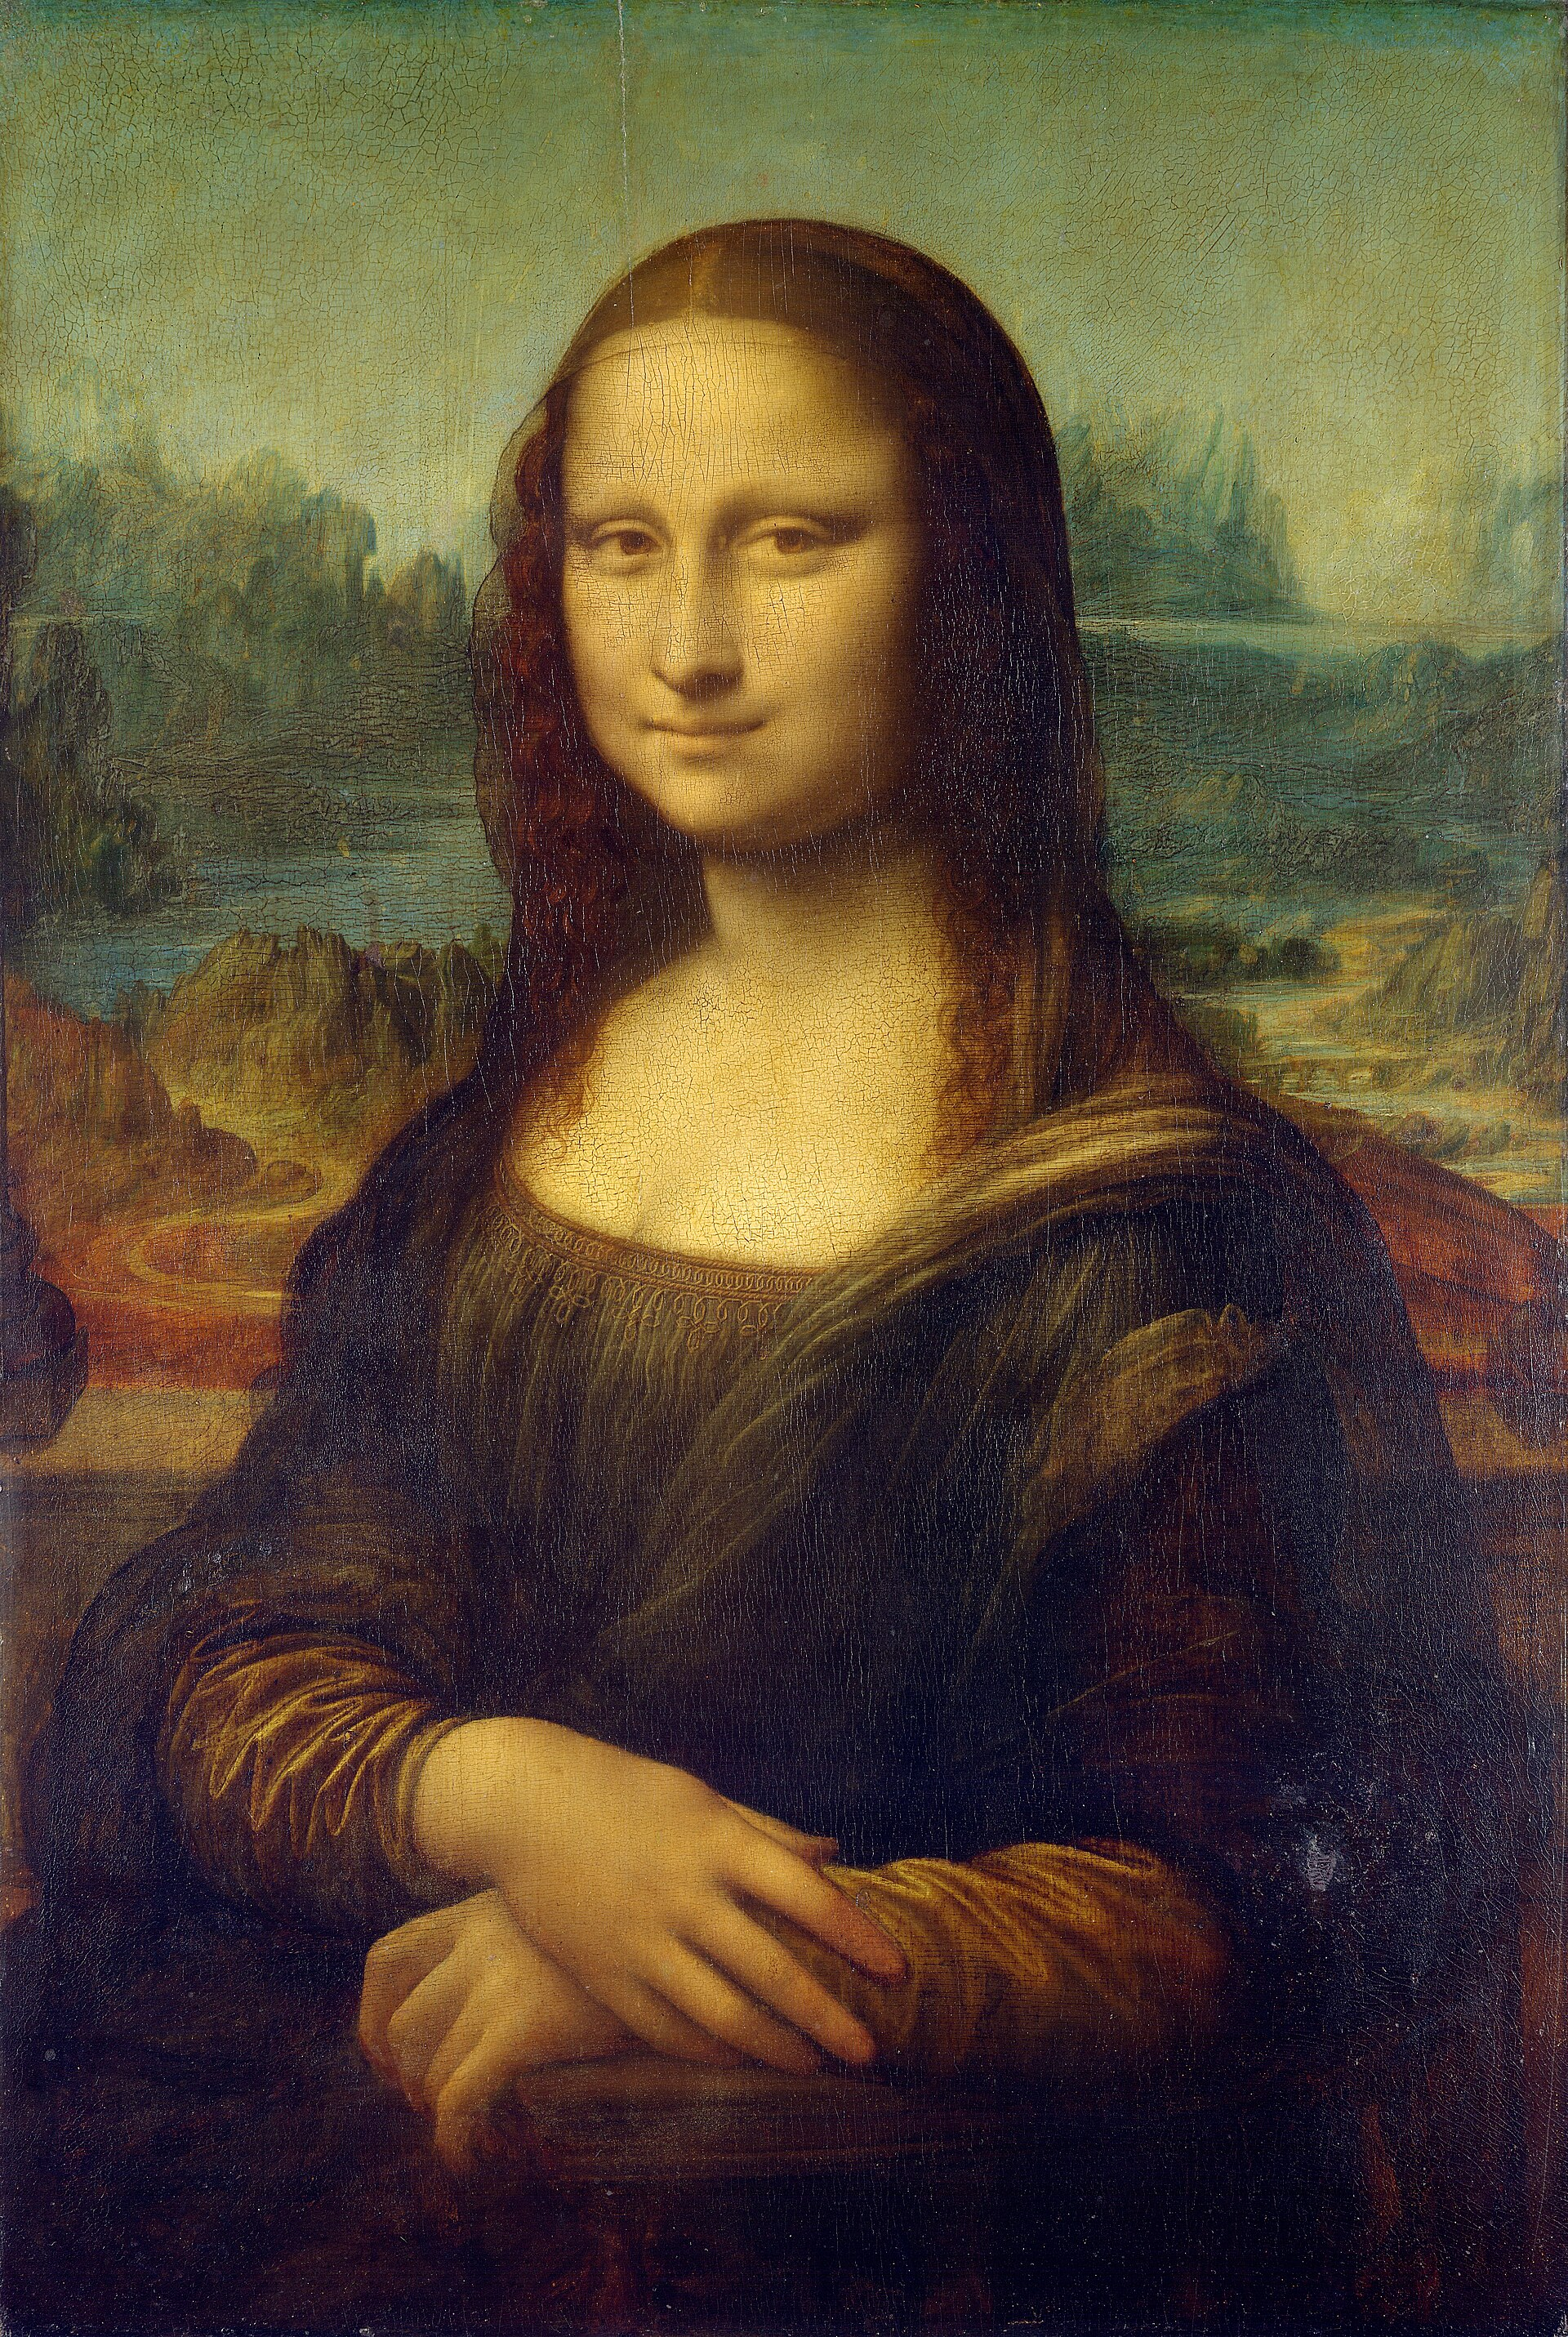
\includegraphics[width=0.5\linewidth]{images/mona_lisa.jpg}
    %\caption{The Mona Lisa, by Leonardo da Vinci}
    %\label{fig:mona_lisa}
%\end{figure}

\section{Week 1 tasks}

\begin{itemize}
    \item $\square$ I have fully read and understood the syllabus.
    \item $\square$ I have fully read and understood the policies and resources listed here:
        \url{https://catalog.arizona.edu/syllabus-policies}.
    \item $\square$ I have fully read and understood the College of Information
        Science Academic Integrity policy:
        \url{https://infosci.arizona.edu/students-and-career/academic-integrity}.
\end{itemize}


\section{Workload}

How many hours did you spend on this assignment outside the classroom?

\section{Acknowledgments}

% Cite all the people you've worked with on this homework.

\end{document}
